\section{Experimental design and results}

\subsection{Dataset Selection}
\label{sec:results:data}

There are morn than thousands of ambugious words in the SemCor corpuse, by our
definition in secton~\ref{sec:formulate:preprocess}, which will translate to
more than thousands of datasets and the corresponding machine learning tasks.
However, not all dataset is qualified for a tractable machine learning problem. 
The problem is that some words have senses that are rarely appeared in the
sencor corpus, which is typically 1 or 2 appearances.
The lack of data makes the word sense unlearnable.
Therefore, we use two criteria to select the set of training set we use in our
experiment:
(1) Overall instances greate than 200, 
and (2) Each sense ids (labels / classes) appear at least 20 times.

\subsection{Parameters Tuning}

\Paragraph{Logistic Regression}
We first perform a parameter search over 5-fold cross-validation over the entire
training set for different words. We tested different regularization values,
solvers, multiclass metrics. Finally we found that in most cases by setting C=1,
solver=``newtown\_cg'', max\_iter = 500, and metric=``multinomial'' we can get
the best accuracy and f1 scores. We'll set them to be the global parameters over
logistic regression classifier for each word. 

\Paragraph{SVM}.
For each type of SVM models, we execute a 3-fold cross-validation on the
training set for choosing the best parameters. The
\texttt{grid\_search.GridSearchCV()} method in \texttt{sklearn} module in Python
is used for this. We maintain the default stratified 3-fold splitting approach
during cross-validation. The parameter to be tuned for Linear SVM is C, for RBF
SVM is \{C, gamma\}, and for Polynomial SVM is \{C, degree\}. The range of
values for each parameter is set as follows.

C = [0.01, 0.1, 1, 10, 100] \\
gamma = [0.0001, 0.001, 0.01, 0.1, 1, 10] \\
degree = [2, 3, 4, 5]

Eventually, for each target word, each type of SVM models has its own tuned best
parameters.

\Paragraph{Neural Network}.
Because the limitation of dataset and purpose of in comparison with other modeling method, the model parameters used in the network for comparison are two dilation blocks with each only two layers to process four words. Only forward processing blocks exist, since the dataset is too small, which has been under-fitting. Number of filters of both causal convolution and dilation layers is 8. Number of filters of dense layer before the softmax layer is 16. Adam was used as the optimizer. The data is trained the whole dataset of a word per batch, and repeated five times for the same dataset. 

\subsection{Results: Weighted F1 Scores}
\label{sec:eval:results}

We use \textbf{weighted} F1 scores to account for the class imbalance effect in
the dataset. 
That is, we first calculate F1 scores for each class, and then average them,
weighted by the number of each class in the test set.

Using the critia in section~\ref{sec:results:data} we filter out the eight words
in evaluation result in figure~\ref{fig:results:f1}.
But these dataset consist too few training instances for our neural network
algorithm to converge.
To evalute the neural network's performance, we loose the second critia (fewer
instance on some minor classes) and include two larger dataset, and results in
figure~\ref{fig:results:f1-large}.
We handle the minor class issues (classes with only one or two labels), by
manually upsampling the instances of such classes to 20.

\begin{figure*}[t!]
    \centering
  \begin{subfigure}[t]{0.68\textwidth}
    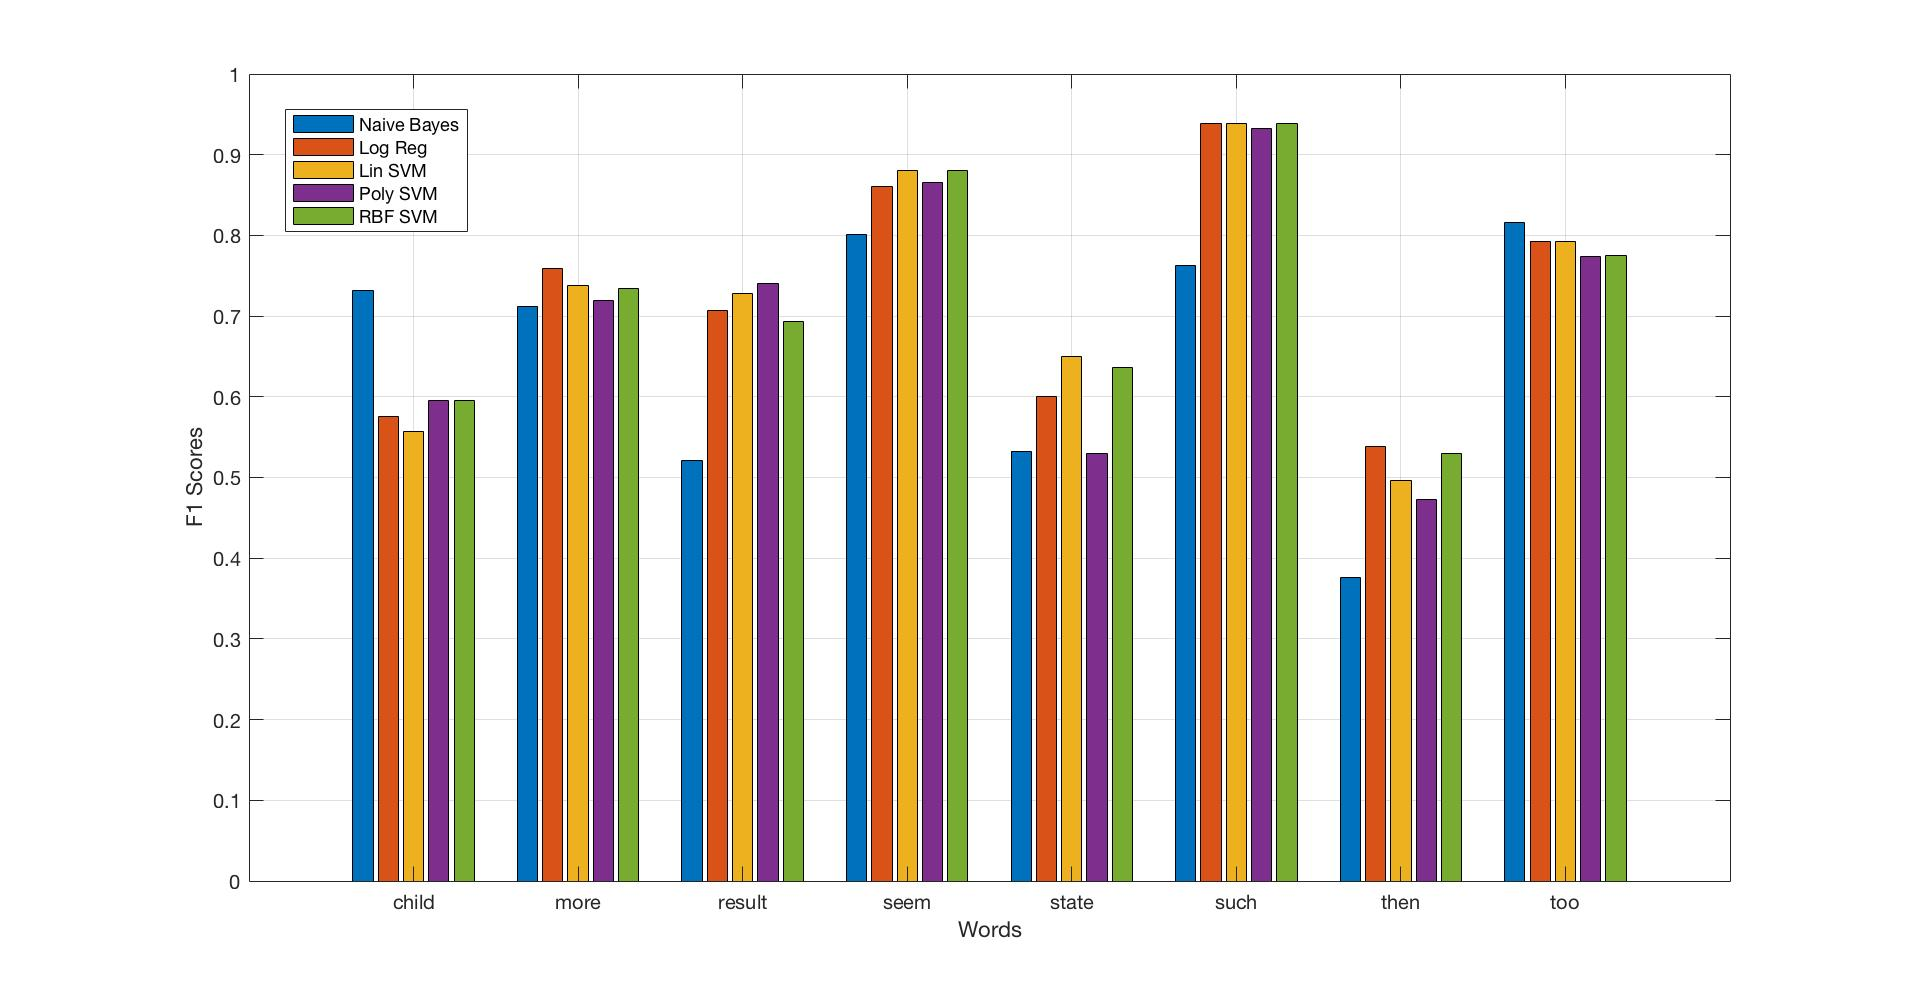
\includegraphics[width=\textwidth]{plots/f1.jpg}
    \caption{Weighted F1 scores on small-scale dataset}
    \label{fig:results:f1}
\end{subfigure}
  \begin{subfigure}[t]{0.3\textwidth}
    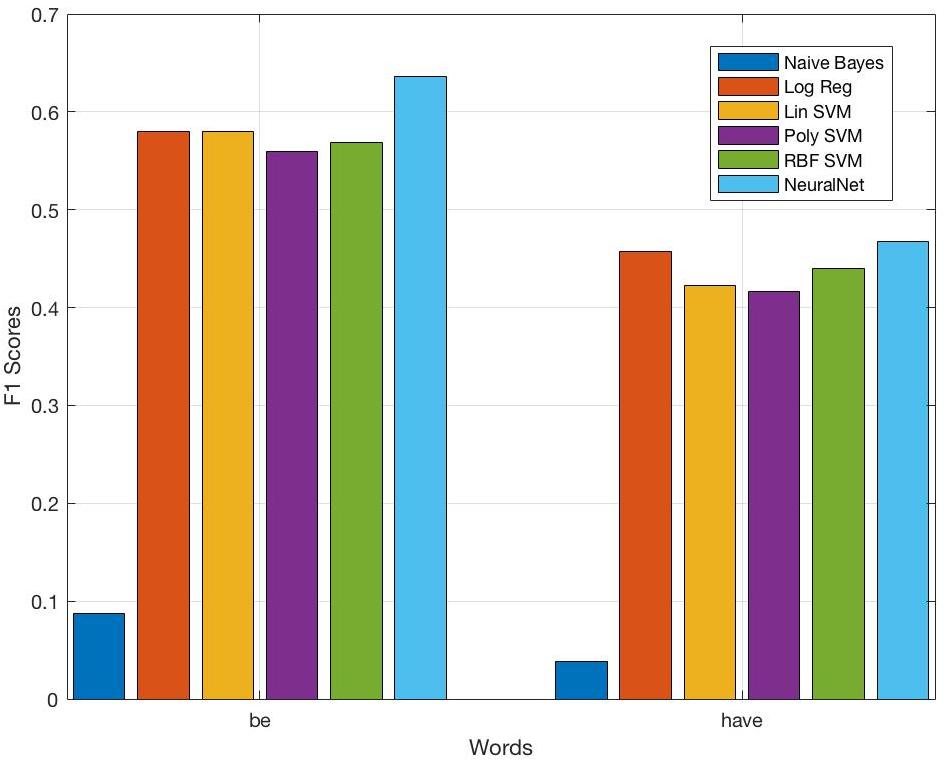
\includegraphics[width=\textwidth]{plots/f1_large.jpg}
    \caption{on larger dataset}
    \label{fig:results:f1-large}
\end{subfigure}
\end{figure*}

\Paragraph{Logistic Regression and SVM works consistently well}
Comparing the bars for Logistic Regression and SVMs, in
figure~\ref{fig:results:f1} and figure~\ref{fig:results:f1-large},
we notice they yields close F1 socres on both small and large dataset.

Kernel method doesn't give significant improvement to SVM.
Neither RBF Kernel SVM and Polynomial Kernel SVM shows better performance over
linear SVM.

\Paragraph{Neural Network dominates large dataset.}
Even though the part of the dataset is synthesized, (upsampling to handle class
imbalance), Neural Network outperforms the rest of the classifiers.

\Paragraph{Naive Bayes only works at small-scale dataset}.
A significant performance downgrade shown on large dataset
(figure~\ref{fig:results:f1-large}).
However, on small dataset, Naive Bayers is able to catch up with the other
discriminative models.

